% !TeX root = ./main.tex

\section{Seat Assignment with Dynamic Demand}
    \frame{\sectionpage}

\begin{frame}{Dynamic Demand}
  \begin{itemize}
    \item[-] There is at most one group arrival at each period, $t = 1, \ldots, T$. 
    \item[-] The probability of an arrival of group type $i$: $p_i$.  
  \end{itemize}

  1. Assign the seats under the fixed seat planning

  \begin{footnotesize}
    The seats, which were arranged for social distancing purposes, need to be dismantled before people arrive to prevent them from occupying those seats. When each group arrives, we make decisions regarding whether to accept or reject them based on the predetermined seat planning.
  \end{footnotesize}

  \vspace{0.3cm}

  2. Assign the seats under the flexible seat planning

  \begin{footnotesize}
  Scenario 1: the seller need to assign seats each time a group arrives. 
  
  Scenario 2: the seller only needs to accept or reject the group's request and then assign the seats after the selling period.
  \end{footnotesize}
\end{frame}

  \begin{frame}{Seat Assignment under Fixed Seat Planning}
    % To evaluate the effectiveness of the initial seat planning, we employ a dynamic situation where decisions are made based on real-time feedback. In this context, we utilize a fixed seat planning as the foundation, and then make informed decisions accordingly.
    \small
    \begin{itemize}
      \item Group-type Control
      \item[-] Obtain the seat planning from stochastic programming. Suppose the corresponding supply is $[X_1, \ldots, X_M]$. ($X_{i} = \sum_{j} x_{ij}, \forall i$)
      
      For the arrival of group type $i$,

      \item[-] if $X_i > 0$, accept it directly, assign it the seats planned for group type $i$;
      \item[-] if $X_i = 0$, determine which group type to accept it.
    \end{itemize}

    % \begin{tiny}
    % Let $D^t_j$ be the random variable indicates the number of group type $j$ in $t$ periods.

    % $P(D_{i}^{T-t} \geq x_i)$ is the probability that the demand of group type $i$ in $(T - t)$ periods is no less than $x_i$.
    % \end{tiny}

    % $d^{t}(i, j)$ = $\underbrace{i + (j-i-\delta)P(D_{j-i-\delta}^{T-t} \geq x_{j-i-\delta}+1)}_{\text{acceptance}}$ - $\underbrace{j P(D_{j}^{T-t} \geq x_{j})}_{\text{rejection}}.$
    \vspace{-0.5cm}

    \begin{figure}[h]
      \centering
      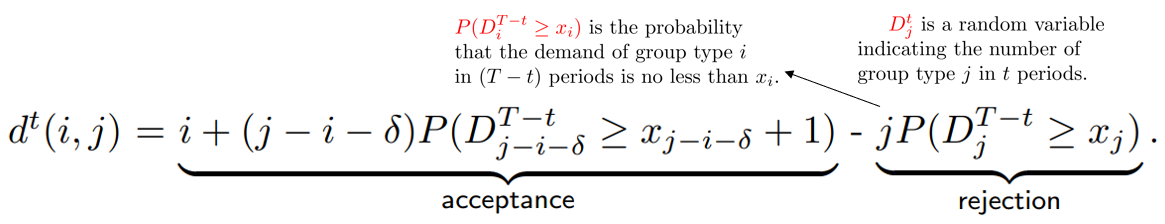
\includegraphics[width = 0.9\textwidth]{./images/d_ij.png}
    \end{figure}

    \vspace{-0.1cm}

    For all $j > i$, find the maximum value denoted as $d^{t}(i, j^{*})$.
    
    If $d^{t}(i, j^{*}) > 0$, we place the group of $i$ in $(j^{*} + \delta)$-size seats. Otherwise, reject the group.

    % After acceptance, customers have more freedom to choose their seats with the seat planning.
  \end{frame}
  
  % \begin{frame}{Group-type Control}
  %   Let $D^t_j$ be the random variable indicates the number of group type $j$ in $t$ periods.

  %   $P(D_{i}^{T-t} \geq x_i)$ is the probability that the demand of group type $i$ in $(T - t)$ periods is no less than $x_i$.
  % \end{frame}

  \begin{frame}{Performance}
    \scriptsize
    The assignment is based on the fixed seat planning and we use the group-type to make the decision. 
    % \begin{table}[ht]
    %     \begin{tabular}{|l|l|l|l|l|}
    %     \hline
    %     \# of samples & T & probabilities & \# of rows & \# of people \\
    %     \hline
    %     1000  & 45  & [0.4,0.4,0.1,0.1] & 8  & 85.3 \\
    %       & 50  &  &   & 97.32 \\
    %       & 55  &  &   & 102.40  \\ % slow
    %       & 60  &  &   & 106.02  \\
    %      & 65  &  &   & 108.84 \\
    %     \hline
    %     1000  & 35  & [0.25,0.25,0.25,0.25] & 8  & 87.08 \\
    %       & 40  &  &   & 101.24 \\
    %       & 45  &  &   & 110.52 \\
    %       & 50  &  &   & 114.39 \\
    %       & 55  &  &   & 117.26 \\
    %     \hline
    %     5000  & 300  & [0.25,0.25,0.25,0.25] & 30  & 749.76 \\
    %      & 350  &  &   & 866.42 \\
    %       & 400  &  &   & 889.44 \\
    %       & 450  &  &   & 916.66 \\
    %     \hline
    %     \end{tabular}
    % \end{table}

    $M =4$, $\delta =1$, $L_j =21, j \in \mathcal{N}$, $p_0 = 0$, $|\Omega| = 1000$.
    \begin{table}[ht]
      \centering
      \begin{tabular}{|l|l|l|l|l|}
      \hline
       T & Probabilities & \# of rows & SSP (\%) & Expected demand (\%) \\
      \hline
      70  & [0.25, 0.25, 0.25, 0.25]  & 10 & 94.97 & 94.71  \\
      80  &   &  & 96.48 & 96.16  \\
      90  &   &  & 97.94 & 97.36  \\
      100  &   &  & 98.91 & 96.27  \\
      \hline
      70  & [0.25, 0.35, 0.05, 0.35]  & 10 & 95.90 & 95.60 \\
      80  &   &  & 97.06 & 96.69 \\
      90  &   &  & 98.58 & 98.58 \\
      100  &   &  & 99.47 & 95.97 \\
      \hline
      70  & [0.15, 0.25, 0.55, 0.05]  & 10 & 97.41 & 96.70 \\
      80  &   &  & 98.85 & 96.06 \\
      90  &   &  & 98.73 & 97.63 \\
      100  &   &  & 98.46 & 98.19 \\
      \hline
      140  & [0.25, 0.25, 0.25, 0.25]  & 20 & 95.83 & 95.78 \\
      160  &   &  & 97.46 & 96.89 \\
      180  &   &  & 99.05 & 96.42 \\
      200  &   &  & 99.74 & 97.57 \\
      \hline
      \end{tabular}
    \end{table}

  % Each entry is the average of 50 instances.
  % IP will spend more than 2 hours in some instances, as `NA' showed in the table.
  \end{frame}

  \begin{frame}{Real-time Seat Assignment}
    \centering
    Dynamic Seat Assignment Problem
    \small
    \begin{itemize}
    \item[-] There is one and only one group arrival at each period, $t = 1, \ldots, T+1$. 
    \item[-] The probability of an arrival of group type $i$: $p_i$.
    \item[-] $\mathbf{L} = (l_1, l_2, \ldots, l_{N})$, where $l_j =0,\ldots, L_j, j\in \mathcal{N}$: Remaining capacity.
    \item[-] $u_{i,j}^{t}$: Decision. Assign group type $i$ to row $j$ at period $t$, $u_{i,j}^t =1$.
    \item[-] $U^{t}(\mathbf{L}) = \{u_{i,j}^{t} \in\{0,1\}, \forall i,j| \sum_{j=1}^{N} u_{i,j}^{t} \leq 1, \forall i, n_{i}u_{i,j}^{t}\mathbf{e}_j \leq \mathbf{L}, \forall i,j \}$.
    \item[-] $\mathbf{e}_j$: Unit column vector with $j$-th element being 1.
    \item[-] $V^{t}(\mathbf{L})$: Value function at period $t$, given remaining capacity, $\mathbf{L}$.
    \end{itemize}

    $$V^{t}(\mathbf{L}) = \max_{u_{i,j}^{t} \in U^{t}(\mathbf{L})}\left\{ \sum_{i=1}^{M} p_i ( \sum_{j=1}^{N} i u_{i,j}^{t} + V^{t+1}(\mathbf{L}- \sum_{j=1}^{N} n_i u_{i,j}^{t}\mathbf{e}_j)) + p_0 V^{t+1}(\mathbf{L})\right\}$$
    \small
\end{frame}

  \begin{frame}{Proposed Methods}
    We make the decision under the flexible seat planning.

    \begin{itemize}
      \item Suppose the supply associated with the seat planning is $[X_{1}, \ldots, X_M]$.
      
      \vspace{0.5cm}

      For the arriving group type $i$,

      \item[-] if $X_i > 0$, accept the group, assign it according to the break tie rule;
      
      \item[-] if $X_i = 0$, different methods:
      
      \vspace{0.5cm}

      1. Based on the adjusted SSP.

      2. Based on the seat planning from the relaxation of SSP.

    \end{itemize}
  \end{frame}

  \begin{frame}{Method 1}
    \scriptsize
    To determine the appropriate row assignment for the current group type $k$, we introduce the decision variables $a_j, j \in \mathcal{N}$ indicating whether we accept it in row $j$.
    
      % \item Obtain the seat planning after the realization of group.
      \begin{tiny}
        \begin{equation}\label{adjusted_SSP}
        \begin{aligned}
        \max \quad & \sum_{j} k a_j + E_{\omega}\left[\sum_{i=1}^{M-1} (n_i-\delta) (\sum_{j= 1}^{N} x_{ij} + y_{i+1,\omega}^{+} - y_{i \omega}^{+}) + (n_{M}-\delta) (\sum_{j= 1}^{N} x_{Mj} - y_{M \omega}^{+})\right] \\
        \text {s.t.} \quad & \sum_{j= 1}^{N} x_{ij}-y_{i \omega}^{+}+
        y_{i+1, \omega}^{+} + y_{i \omega}^{-}=d_{i \omega}, \quad i = 1,\ldots,M-1, \omega \in \Omega \\
        & \sum_{j= 1}^{N} x_{ij} -y_{i \omega}^{+}+y_{i \omega}^{-}=d_{i \omega}, \quad i = M, \omega \in \Omega \\
        & \sum_{i=1}^{M} n_{i} x_{ij} \leq L_j - n_k a_j, j \in \mathcal{N} \\
        & \sum_{j=1}^{N} a_j \leq 1 \\
        & x_{ij} \in \mathbb{Z}_{0}^{+}, \quad i \in \mathcal{M}, j \in \mathcal{N}, y_{i \omega}^{+}, y_{i \omega}^{-} \in \mathbb{Z}_{0}^{+}, \quad i \in \mathcal{M}, \omega \in \Omega,  a_j \in \{0,1\}, j \in \mathcal{N}.
        \end{aligned}
      \end{equation}
    \end{tiny}
    \begin{itemize}      
      \item[-] If $X_i = 0$, solve problem \eqref{adjusted_SSP}, make the decision and update the seat planning.
    \end{itemize}
  \end{frame}

  % \begin{frame}{Method 2 Overview}
  %   \begin{itemize}
  %     \item Obtain the seat planning composed of full or largest patterns.
      
  %     - Obtain the optimal solution from the relaxed SSP
      
  %     - Integral seat planning from deterministic model
  
  %     - Construct largest or full patterns.
  
  %     \vspace{0.5cm}

  %     \item Dynamic seat assignment
  
  %     - Determine the group type by group-type control
  % % Tell us which group type should be broke which determines which rows can be placed. 
  
  %     - Decision on assigning the group to a specific row

  %   \end{itemize}
  % \end{frame}
    

% \begin{frame}{Construction}
% There exists an optimal solution to the stochastic programming problem such that the patterns associated with this optimal solution are composed of the full or largest patterns under any given scenarios.
% \end{frame}

    \begin{frame}{Method 2: Dynamic Seat Assignment (DSA)}
      If $X_i = 0$,
      
      1. Determine the group type $j^{*}$ by the group-type control.

      2. Make the decision on assigning the group to a specific row.
      \begin{itemize}
        \item Break tie for determining a specific row
        \item Decision on assigning the group
        \item[-] Value of Acceptance (VoA): value of LP relaxation of SSP with $(\mathbf{L}-n_i \mathbf{e}_{j^{*}})$ plus $i$.
        
        % approximation of $V_{t} (\mathbf{L}-n_i \mathbf{e}_{j^{*}})$ + $i$. 
        % approximation of $V_{t} (\mathbf{L})$

        \item[-] Value of Rejection (VoR): value of LP relaxation of SSP with $\mathbf{L}$.

        \item[-] If VoA is no less than VoR, accept group type $i$; otherwise, reject it.
      \end{itemize}
      Regenerate the seat planning
      \begin{itemize}
      \item[-] When $X_{M} =0$
      \item[-] When comparing VoA and VoR 
      \end{itemize}
    \end{frame}

    \begin{frame}{Compared with Other Policies}
      We have the following policies compared with DSA when we make the instant allocation.
      
      \vspace{0.5cm}
      
      \begin{itemize}
        \item Bid-price control
        \item Dynamic programming based heuristic
        \item Booking limit control
        \item First come first served
        \item[-] Optimal: full knowledge of demands
      \end{itemize}
    \end{frame}

      \begin{frame}{Bid-price Control}
        The dual problem of LP relaxation of problem \eqref{deter_upper} is:
        \begin{equation}\label{bid-price_dual}
          \begin{aligned}
          \min \quad & \sum_{i=1}^{M} d_i z_i + \sum_{j= 1}^{N} L_j \beta_{j} \\
          \text {s.t.} \quad & z_{i} + \beta_j n_i \geq (n_i-\delta), \quad i \in \mathcal{M}, j \in \mathcal{N} \\
          & z_{i} \geq 0, i \in \mathcal{M}, \beta_{j} \geq 0, j \in \mathcal{N}.
          \end{aligned}
        \end{equation}
        
        \small
        
        The optimal solution to problem \eqref{bid-price_dual} is given by $z_1, \ldots, z_v =0, z_i = \frac{\delta (n_i - n_v)}{n_v}$, for $i = v + 1, \ldots, M$, $\beta_j = \frac{n_v - \delta}{n_v}$ for all $j$.
        \vspace{0.5cm}

        For the group type $i$, if $i - \beta_j n_i \geq 0$, accept it. 
        % The bid-price control policy will make the decision to accept group type $i$, where $i$ is greater than or equal to $h$, if the capacity allows.
      \end{frame}

      \begin{frame}{Dynamic Programming Based Heuristic}
        \begin{itemize}
        \item Relax all rows to one row with the same capacity by $L = \sum_{j=1}^{N} L_j$.
        \item[-] Deterministic problem: $\{\max \sum_{i=1}^{M} (n_i- \delta) x_{i}: x_{i} \leq d_{i}, i \in \mathcal{M}, \sum_{i=1}^{M} n_{i} x_{i} \leq L, x_{i} \in \mathbb{Z}_{+}\}$.
        \item Decision: $u^{t}$. If we accept a request in period $t$, $u^t = 1$; otherwise, $u^t =0$.  
        \item[-] DP with one row can be expressed as:
        $$V^{t}(l) =  \max_{u^{t} \in \{0,1\}} \left\{ \sum_{i} p_i [V^{t+1}(l-n_i u^{t})+ i u^{t}] + p_0 V^{t+1}(l)\right\}, l \geq 0 $$

        $$V^{T+1}(l) =0, \forall l.$$
        \item After accepting one group, assign it in some row arbitrarily when the capacity of the row allows.
        \end{itemize}
      \end{frame}
      
      \begin{frame}{Booking limit Control}
        Basic idea: for each type of requests, we only allocate a fixed amount according to the static solution and reject all other exceeding requests.
        \begin{itemize}
          \item[1] Observe the arrival group type $i$.
          \item[2] Solve problem \eqref{deter_upper} using the expected demand.
          \item[3] Obtain the optimal solution, $x_{ij}^{*}$ and the aggregate optimal solution, $\mathbf{X}$.
          \item[4] If $X_{i} > 0$, accept the arrival and assign the group to row $k$ where $x_{ik} > 0$, update $\mathbf{L}^{t+1} = \mathbf{L}^{t} - n_i \mathbf{e}_{k}$; otherwise, reject it, let $\mathbf{L}^{t+1} = \mathbf{L}^{t}$.
        \end{itemize}
                 
        % When we solve the linear relaxation of problem \eqref{deter_upper}, the aggregate optimal solution is the limits for each group type. Interestingly, the bid-price control policy is found to be equivalent to the booking limit control policy.
      \end{frame}